\chapter{Implementation}

Despite what was thought to be a reasonable list of features for a minimal implementation, the actual act of implementing them proved to be a lot tougher than anticipated, with a lot of problems arising that were completely unforeseen. The server in particular proved to be a serious problem, though the client was not without it's share of issues as well.

This chapter will go into detail about some of the features implemented in the game. In particular it talks about the graphics renderer, the input and movement handling systems and the server, including a lot of the problems that were encountered and what they meant for the project.

\section{The Game Loop}\label{game_loop_implementation}
There are several important parts of the game engine that exist outside its purview, but all the fundamental game logic works on a per-frame basis, and those frames are defined and controlled by the game loop.

Traditionally the game loop is defined as a \texttt{while} loop, which runs until a flag is unset saying the game is over and it's time to shut down. However, in a JavaScript browser game this won't work. The reason for this is that a \texttt{while} loop is blocking, and if the browser is blocked it won't be able to perform other functions on the page, such as displaying the output of the renderer, or registering input from the user.

Because it is not possible to let the game loop take complete control of the browser thread using a \texttt{while} loop another method has to be used to run the game loop instead. The method chosen is the use of the \texttt{setInterval()} function built into JavaScript, which will repeatedly call a function given to it after a given interval. Because the design has the game loop running at 30 frames per second, this means that the interval is 33.3 milliseconds. The interval itself isn't directly given as 33.3 milliseconds, however. Rather, it is contained within a variable called \texttt{UPDATE\_INTERVAL}. This of course has the advantage of letting the frame duration value be used anywhere, and can be changed easily to another value any time.

This timing works perfectly well and as long as a frame is always able to be processed in the 33.3 milliseconds it needs nothing will go wrong. However, if for any reason a situation arises where a frame takes longer than that to be processed there will be issues and the timing will be thrown off.

A really good example of something that causes the timing to be thrown off like this is a feature modern browsers have that pauses or slows down repeated events in tabs that are not in focus. This essentially has the effect of causing a frame to take a very long time to process---potentially for as long as it takes for a user to switch back to the tab. Without any way to handle this delay the game loop will be behind where it should be. This means that when the user returns to the tab the game loop will start running at the correct speed again and whatever happened will be played back behind when it actually happened. In a single player game this pausing effect might be desirable\footnote{Though it is a bad idea to rely on this to be an actual pausing feature, as it might not be present in all browsers, or function the same across those that do implement it.}, but in a multiplayer game this causes the user to be completely desynchronised from the actual state of the game.

\noindent
\begin{minipage}{\linewidth}
\begin{lstlisting}[style=js, caption={The client-side game loop.}, label=game_loop]
function tick() {
    var entities = this.scene.getEntities();

    var current_time = Date.now();
    var elapsed_time = current_time - this.previous_time;
    this.previous_time = current_time;
    this.lag += elapsed_time;

    while (this.lag >= UPDATE_INTERVAL) {
        for (var i = 0, len = entities.length; i < len; i++) {
            entities[i].update(this);
        }
        this.lag -= UPDATE_INTERVAL;
    }

    this.scene.setEntities(entities);

    this.network.update();
}
\end{lstlisting}
\end{minipage}


To solve this the game loop keeps track of when it was last run and the lag that is caused by the difference between the previous run and the current run. There are two variables kept in the \texttt{Engine} class that are used for this. The first is \texttt{previous\_time}, which is what records the previous run time. The second is \texttt{lag}, which is used to catch up if a frame has taken longer than expected to complete. Every time a frame is processed the loop works out the time elapsed between the previous and current run and then adds this to \texttt{lag}. There is then a \texttt{while} loop that runs while the value of \texttt{lag} is greater than or equal to the value of \texttt{UPDATE\_INTERVAL}. This has the effect of both not updating a frame too soon---though for the most part that is handled by \texttt{setInterval()}---and also making sure the game loop doesn't fall behind by running through all the updates until it has caught up. The only downside to this is that if frames are always taking longer to process than they should the game will get stuck always trying to catch up. However, in that case it is necessary to either turn down the frequency of updates or optimise until frames can be processed quickly enough.

\section{Renderer}
The graphics renderer was the first piece of the game engine worked on. Having the graphics to provide a view into the game world was important in order to easily see whether things were behaving as expected and proved extremely useful in detecting problems with other parts of the game later on.

This section will go over firstly what isometric projection is and then the ways that graphics are actually drawn to the screen. Finally, the difficulties that the renderer caused during implementation will be discussed.

\subsection{Isometric Tiles}

\subsubsection{What Is Isometric?}
When talking about isometric projection in the videogame world it is important to know that it is not truly isometric. True isometric requires that all three coordinate axes are equally foreshortened. What the gaming world calls `isometric' is in fact \textit{dimetric} projection---a projection where two axes are equal but the third is not.

The reasons for doing this are essentially one of aesthetics when drawing objects at a very low resolution with visible pixels. At these very coarse resolutions true isometric projection creates an aesthetically displeasing line. However, by changing to a dimetric projection, where the line grows twice as fast horizontally as it does vertically, the line becomes much more consistent and visually appealing.

\begin{figure}[H]
    \centering
    
\includegraphics[width=8cm]{Images/iso_dimetric.eps}
    \caption{The line of the left represents isometric projection, the line on the right dimetric.}
    \label{fig:iso_dimetric}
\end{figure}


\subsubsection{Cartesian To Isometric}
The term ``\textsc{2d} isometric tile'' used in this report is a little ambiguous. The game world itself is represented by simple \textsc{2d} Cartesian coordinates that map to a grid of tiles. Isometric space, however, is \textsc{3d}. The term used here refers to the type of graphic used to represent the tiles in isometric space, rather than the isometric space itself. These graphics are simple \textsc{2d} images, drawn in such a way as to make them look \textsc{3d}.

\begin{figure}
    \centering
    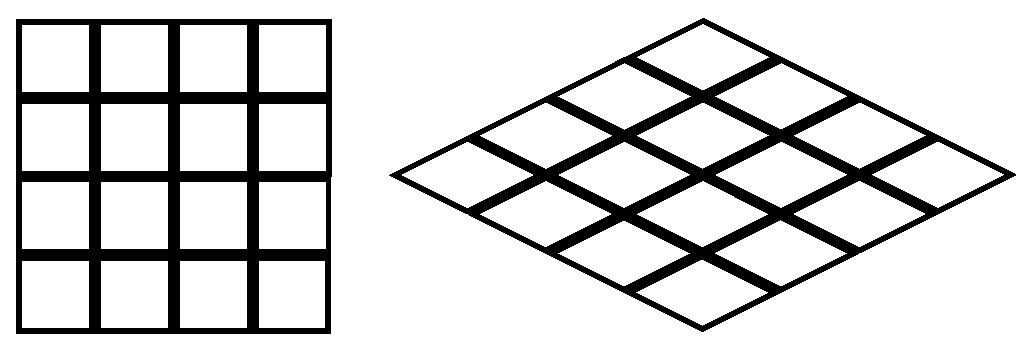
\includegraphics[width=8cm]{Images/cart_iso_grid.eps}
    \caption{A \textsc{2d} grid and an isometric grid.}
    \label{fig:cart_iso_grid}
\end{figure}

Of course, this means that a conversion has to be made between the two coordinate systems in order for the renderer to be able to display things in their proper place. As an example, figure \ref{fig:map_without_iso_coords} shows what the game world looks like if it is rendered without this coordinate conversion---clearly very wrong.

\begin{figure}[H]
    \centering
    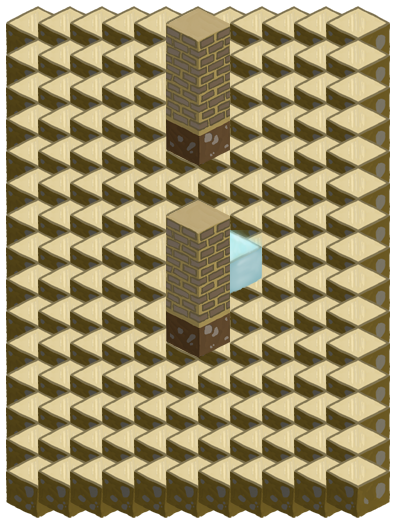
\includegraphics[height=5.8cm]{Images/map_without_iso_coords.png}
    \caption{The ingame map rendered without first converting to isometric coordinates.}
    \label{fig:map_without_iso_coords}
\end{figure}


In order for the renderer to show things correctly in the isometric space there needs to be a way of converting between the game world's Cartesian coordinates and the renderer's isometric coordinates. Luckily, this is incredibly simple:

\noindent
\begin{minipage}{\linewidth}
\begin{lstlisting}[style=js, caption={JavaScript implementation of a function to turn Cartesian coordinates into game isometric coordinates. Original algorithm from \cite{citeulike:13155325}.}, label=cartesian_to_isometric]
function cartesianToIsometric(cartesian_x, cartesian_y)
{
	var isometric = {};

    isometric.x = cartesian_x - cartesian_y;
    isometric.y = (cartesian_x + cartesian_y) / 2;

    return isometric;
}
\end{lstlisting}
\end{minipage}

Now when the renderer draws the game to the \textsc{html5} canvas, it can first call the \texttt{cartesianToIsometric} function, letting it place the tile graphics in the correct place as seen in figure \ref{fig:map_with_iso_coords}.

\begin{figure}
    \centering
    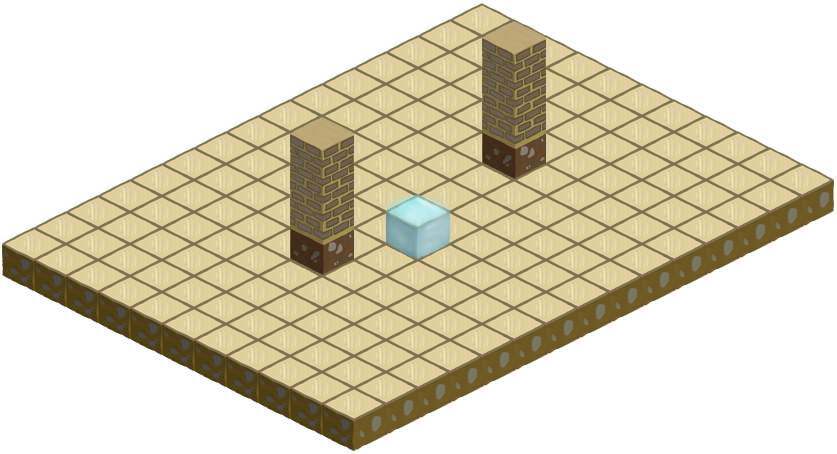
\includegraphics[width=8cm]{Images/map_with_iso_coords.png}
    \caption{The ingame map rendered with the conversion to isometric coordinates.}
    \label{fig:map_with_iso_coords}
\end{figure}

\subsection{Rendering}
After the renderer has converted between Cartesian and isometric spaces it needs to be able to draw things to the canvas. The actual drawing of a game tile to the canvas is straightforward, simply requiring a call to the canvas' \texttt{drawImage()} function and supplying it the image you wish to draw and the canvas coordinates for where you wish it to be drawn.

The difficult part comes before that. Firstly, you need to be able to work out what the canvas coordinates are. The conversion between isometric coordinates and the canvas coordinates works as follows:

\noindent
\begin{minipage}{\linewidth}
\begin{lstlisting}[style=js, caption={Conversion between isometric coordinates and canvas coordinates.}, label=isometric_to_canvas]
canvas_x = isoCoords.x * (TILE_WIDTH / 2);
canvas_y = isoCoords.y * (TILE_HEIGHT / 2) - (image_height - (TILE_HEIGHT / 2));
\end{lstlisting}
\end{minipage}

A few things should be explained about this. Firstly, \texttt{TILE\_WIDTH} and \texttt{TILE\_HEIGHT} refer to the set size of a single tile and are used to work out the tile's positioning in the world. The \texttt{image\_height} value refers to how tall in pixels an image is. Theoretically an image can have any size and isn't limited to how large a tile is. However, in practical terms, an image can only be arbitrarily tall; width needs to be kept within the tile limits or there will be problems with depth sorting, for reasons seen in Section \ref{depth_limits}.

\begin{figure}[H]
    \centering
    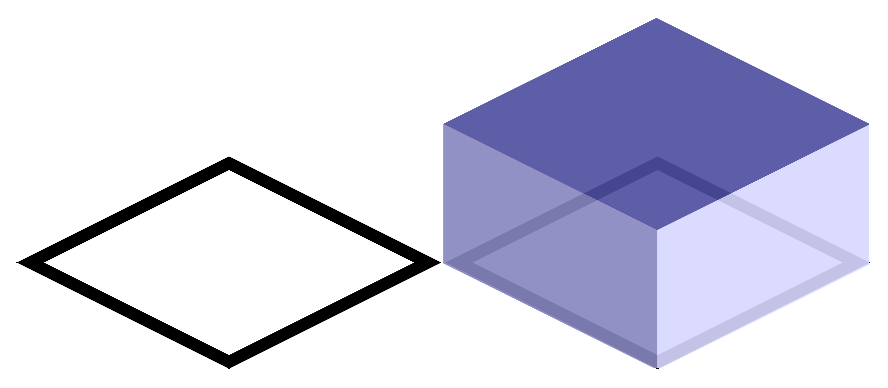
\includegraphics[width=8cm]{Images/tile_and_image.eps}
    \caption{The left shows a tile position. The right shows an image occupying that tile position.}
    \label{fig:tile_and_image}
\end{figure}

Once you have the coordinates you then need to get the tile graphic to use as the image being rendered. Getting the image itself is a very simple task, but getting the order in which to draw them right is more difficult. The \textsc{html5} canvas is a very simple element and it has no ability to specify the relative depth of things being drawn to it; whatever is drawn first will be occluded by what comes afterwards if they overlap. This overlapping is often not a problem when drawing simple \textsc{2d} tiles with a top-down or side-on perspective. However, because the isometric perspective is \textsc{3d} the issue of depth becomes an important one.

\begin{figure}[H]
    \centering
    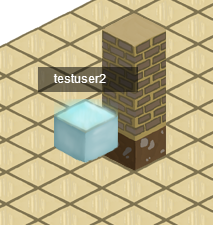
\includegraphics[height=6cm]{Images/broken_depthsort.png}
    \caption{Broken depth sorting.}
    \label{fig:broken_depthsort}
\end{figure}


There are two methods for solving this used in the renderer: a simple painter's algorithm and a depth sorting algorithm. The first is used for the terrain and the second for entities.

\subsubsection{Terrain Rendering}
The terrain is very simple to render as far as isometric projection goes. Terrain images are the same size as the tiles, which means that as long as they are drawn in order the images will never overlap.

The method for achieving this ordering is known as a painter's algorithm\footnote{The painter's algorithm is so called because of a common painting technique whereby distant parts are painted before closer parts that might cover them.} and is very simple. Firstly, all the terrain is stored in a pre-sorted, two dimensional array. Columns are labelled \texttt{y} and rows are labelled \texttt{x}. Images are drawn by looping through each row in each column and drawing them one by one, rendering the images from back to front, row by row.

\begin{figure}[H]
    \centering
    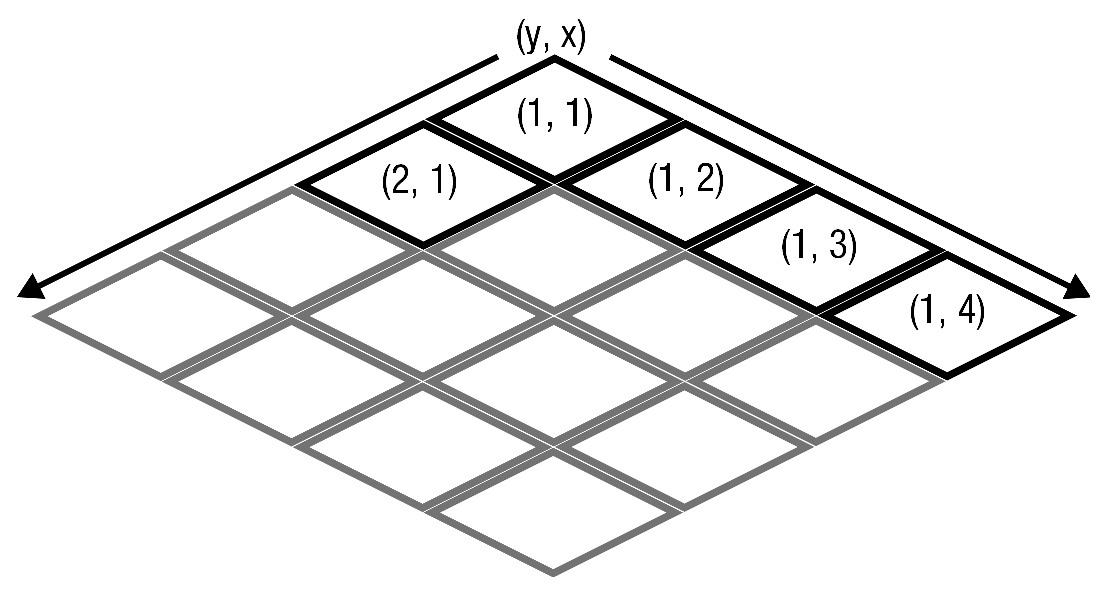
\includegraphics[width=8cm]{Images/painters_algo.eps}
    \caption{The painter's algorithm.}
    \label{fig:painters_algo}
\end{figure}

This is a very efficient and cheap way to render the images to the screen, and works perfectly for the terrain. Even if the terrain were to be made no longer flat, as long as it never broke out of the tile grid there would be no need to change how it is rendered.

\subsubsection{Entity Rendering}\label{entity_rendering}
Unfortunately, entities are less easy to deal with. At least some entities can move around---crossing tile boundaries when they do so---which means they cannot be stored in the same grid that makes up the tiles themselves. Because entities can exist outside of the tile boundaries, working out their depth cannot be done just by iterating through them like the terrain. Another way has to be devised in order to render them in the correct order.

To figure out the order that entities need to be rendered it is first necessary to work out what their relative depth in the scene is. To get an entity's depth, the following calculation is used:

\noindent
\begin{minipage}{\linewidth}
\begin{lstlisting}[style=js, caption={Calculation to work out an entity's relative depth in the scene.}, label=calculate_depth]
function calculateDepth(entity) {
    return Math.round((entity.x * TILE_WIDTH / 2) + (entity.y * TILE_HEIGHT / 2) + entity.z);
}
\end{lstlisting}
\end{minipage}

In this calculation the most important part is the addition of an entity's position data, \texttt{x}, \texttt{y} and \texttt{z}. The \texttt{z} attribute is not currently used in the game, but if it were it would represent relative height from the ground plane and is thus important to the depth calculation. The use of the \texttt{TILE\_HEIGHT} and \texttt{TILE\_WIDTH} attributes is due to the small values of the position data. Because tiles can potentially have small values like \texttt{(1, 1)} it is often common for depth values to be worked out as being the same. Multiple entities sharing a depth value will often cause them to be rendered in the wrong order. The other issue is that positions can be non-integer, such as \texttt{(1.250, 1)}. The sorting method used can't handle this, so it's necessary to round to a whole number in order to make sure it doesn't break.

The sorting method itself is a modified pigeonhole sort, as shown in Listing \ref{depth_sort}.

\noindent
\begin{minipage}{\linewidth}
\begin{lstlisting}[style=js, caption={Depth sorting entities in a scene using a modified pigeonhole sort.}, label=depth_sort]
function depthSort(entities) {
    var buckets = [];

    for (entity in entities) {
        var depth = this.calculateDepth(entities[entity]);

        if (!buckets[depth])
            buckets[depth] = [];
        buckets[depth].push(entities[entity]);
    }

    var result = [];

    for (bucket in buckets) {
        for (entity in buckets[bucket]) {
            result.push(buckets[bucket][entity]);
        }
    }

    return result;
}
\end{lstlisting}
\end{minipage}

The pigeonhole sort works well for this task. The first reason for this is that the number of entities and number of keys are almost always the same, and even when not the smaller number of keys does not affect the performance of the sort. The number of entities being placed into the sort is also usually very small, which means that memory is not a concern, though with a very large number of entities the memory footprint could be a problem. The other reason the pigeonhole sort works well is that it keeps intact the link between a depth value and the entity it represents without any extra work. This means that the sorted array containing the entities can be used directly in the renderer, saving development and processor time.

\subsubsection{Depth Sorting Limitations}\label{depth_limits}
The depth sorting used in the project works well and performs as expected. However, it has a major limitation in that it will not work for entities that can exist across multiple tiles. Currently, all entities are the size of a single tile---though they may have arbitrary height within it. This makes calculating the depth a simple case of looking at position. If an entity were to be larger than a single tile, however, the position data alone would not be sufficient to determine depth.

Although this can be somewhat worked around by simply filling multiple different tiles with entities that contain a different sprite, it is annoying to do so from a content-creation perspective, and only works for static entities. The better option here is to keep a model of an entity's position in \textsc{3d} space. Although the entities themselves are rendered with \textsc{2d} images, because of the isometric projection they still exist in \textsc{3d} space. By keeping data that models this three dimensionality it is possible to work out the depth of an entity without associating it with more than one tile. Instead, it is given a central tile and the data about its size fills out the rest of it.

This approach affects more than just the rendering. By having an actual size in \textsc{3d} space entities can be interacted with in a more fine-grained way. For example, the current system of collision detection simply checks to see whether a tile position contains an entity or not. This is relatively simple to implement but it is not very versatile---position data is very coarse. By turning the game world into a \textsc{3d} simulation it is suddenly possible for position data to be more fine-grained. Not only can the renderer work out the depth of something that is not bound by whole tiles, collision detection is no longer bound by whole tiles either.

Of course, doing this is very complicated and would require a complete rewrite of almost all of the game engine's underlying systems. Given the difficulties already encountered when implementing what was there it was decided that the huge effort involved was not worth it.

\subsubsection{Renderer Control}
All the renderer's work should preferably be done quickly enough that it can show every frame. However, it is also a good idea to not tie the renderer to the game loop itself. This is because the renderer almost always represents the most intense work done by the game, and including it in the main game loop could easily cause frames to take too long to process, causing breakages\footnote{Though in this particular case the load is so light that it would only be a problem on the very oldest hardware.}. In order to solve this the renderer is instead given its own loop that attempts to update as fast as possible but with less priority than the main game loop. This means that if the renderer is proving too difficult to process at 30 frames per second it won't affect the game logic.

The actual implementation of this ability is handled by a function built into modern browsers, called \texttt{requestAnimationFrame()}. This asks the browser to run whatever function is passed into it at the next available opportunity. Because this is not a repeated task like \texttt{setInterval()}, the function passed in itself calls \texttt{requestAnimationFrame()}, and then asks the renderer to draw a frame, thus operating in a recursive fashion.

\subsection{Renderer Implementation Difficulties}
Being the first major feature to be worked on meant that the renderer was subject to a lot of change and iteration as the project developed. Things that appeared to be working fine at first turned out to be inadequate when other features were added. The renderer was probably the most rewritten and refactored part of the entire code base.

The terrain has been the most stable part, with the rendering method being unchanged since it was first implemented. However, the entity rendering was changed a great deal. The initial implementation had the entities rendered in a way similar to the terrain, by placing them into an array at the correct locations and then iterating through it. While this technically worked, it was ugly and was soon found to be completely inadequate once entity movement was introduced to the game.

The method for rendering entities including the depth sorting also did not work perfectly the first time either. At first the pigeonhole sort was not working properly, as entities were overwriting each other when they had the same depth value. This was solved by introducing the idea of buckets that could store multiple entities at once when they had the same depth value. The next step to solving this was to make sure that the depth values weren't so small. Because the depth value needed to be rounded in order to not break the sorting function it was often the case that entities were sharing the same depth value. Although this rarely affected entities that were sitting still in a tile, entities moving around next to others were regularly having their depth be calculated incorrectly. This was solved by adding the tile values to the calculation, which created much more variation in depth and meant the rounding was less significant. It is now far rarer for entities to share a depth value, and when they do they do not overwrite each other.

Beyond these specific problems, the renderer's place as first feature implemented also suffered from the lack of experience, in JavaScript, use of the \textsc{html5} canvas and games programming in general. A lot of time was spent researching and iterating on things that now would be much easier to implement and be done in a lot shorter time.

\section{Input and Movement}
Movement is one of the most important user facing features of the project. It also makes use of several parts of the game engine to work properly, relying on the game loop functioning correctly to advance the entity at the correct pace, the renderer to display this movement across tiles correctly and both the input manager and network manager to receive (and send) commands.

This section will discuss how input is handled and how that relates to movement, as well as how movement works. In both cases, problems that arose during implementation will be covered, as well as how those problems were solved.

\subsection{Input}\label{input_implementation}
The first and most important of these major parts is the input handler. Originally, the input handler was contained entirely in the \texttt{Engine} class. However, with the advent of the event manager it was refactored out into its own class.

Input in the game is mouse-based, rather than keyboard-based. Being mouse-based, input is a little more difficult to handle than if it were possible to simply capture a button press. It is necessary to work out what location exactly the player has clicked, then go through a series of functions to turn the click location into game-world coordinates. Once the coordinates are known, they need to be checked for validity and then passed on, along with the event type, to any entities that might care to know about it.

The first step in this is capturing the user's input. Browsers are helpful in that they keep track of where the user has clicked, which means that the browser event can be captured and used for the game's purposes. To listen for user clicks, a click event listener is attached to the game's canvas. Unfortunately, however, despite being attached to the canvas, the click event coordinates are global and in the context of the window, rather than being local to the canvas. What this means is that click coordinate \texttt{(0,0)} is not, in fact, the corner of the canvas, but instead the corner of the browser window that contains the canvas.

To solve this it is necessary to work out the click's position relative to the canvas. This is accomplished using the code in Listing \ref{canvas_click_coordinates}.

\noindent
\begin{minipage}{\linewidth}
\begin{lstlisting}[style=js, caption={Transforming a user's click to be relative to the canvas, rather than the window.}, label=canvas_click_coordinates]
canvasPosition.x = ((event.clientX - this.engine.camera.x) - this.engine.canvas.offsetLeft) - (TILE_WIDTH / 2);
canvasPosition.y = ((event.clientY - this.engine.camera.y) - this.engine.canvas.offsetTop);
\end{lstlisting}
\end{minipage}

There are a few things to note in this code. First of all, the \texttt{event} used here is the one passed in from the click event listener, and is an object supplied by the browser. The next thing to note is the \texttt{camera} object. This is a game object that acts as the user's viewport into the world. Because the world can be bigger than the canvas itself, it is necessary to have a method of moving the view around the world, which is where the camera comes in. The camera object has an offset, which the renderer takes into account when positioning entities onto the canvas. Of course, this offset needs to be taken into account when detecting where, exactly, the user has clicked in the world, and so it is used here to do that. The coordinates are then set to be relative to the canvas instead of the window by using the \texttt{offsetLeft} and \texttt{offsetTop} values on the canvas itself, which refer to the canvas' position in the browser window.

After this, a set of functions are used to first transform the canvas' isometric coordinates into \textsc{2d} Cartesian coordinates, and then from there to turn those into actual tiles, shown in Listing \ref{iso_cart_tile_coords}.

\noindent
\begin{minipage}{\linewidth}
\begin{lstlisting}[style=js, caption={Turning the canvas isometric coordinates into \textsc{2d} Cartesian coordinates and then into tile positions. Original algorithm to transform isometric to Cartesian space from \cite{citeulike:13155325}.}, label=iso_cart_tile_coords]
var cartCoords = (function(x, y){
    var coords = {};
    coords.x = (2 * y + x) / 2;
    coords.y = (2 * y - x) / 2;
    return coords;
})(canvasPosition.x, canvasPosition.y);

var tileCoords = (function(x, y){
    var coords = {};
    coords.x = Math.floor(x / (TILE_WIDTH / 2));
    coords.y = Math.floor(y / (TILE_WIDTH  / 2));
    return coords;
})(cartCoords.x, cartCoords.y);
\end{lstlisting}
\end{minipage}

With the tile coordinates acquired, they are sent into a method to work out what to do with them. It first checks for the validity of the tile coordinate by checking whether it is inside the bounds of the map. Assuming the coordinates are in bounds, a check is then done to see whether the player has clicked on an entity or whether they have clicked on a terrain tile. Clicking on an entity could mean either an invalid click location or a command to change to controlling that entity, depending on whether the user is the Game Master or not. Clicking on an empty tile---that is, one not occupied by an entity---is a movement command. Holding shift while clicking on an entity is a swap-to-entity command, available only to the Game Master and only for entities that are not already controlled by another player.

\subsection{Movement}
There are two methods of giving an entity a movement command. The first is from the direct input as detailed in the previous section. The other is input from the network. These work similarly but not entirely the same.

When handling input, all moveable entities are subscribed to events for both direct input and network input. Whether they do something with the direct or network input depends on the component they are using to handle it. For a player character, a component to handle the direct input event is used; for a remote character a component to handle the network event is used instead.

\subsubsection{Pathfinding}
With the movement event processed, a series of other methods are called to actually move the entity. The first step is the pathing step, which makes use of the other changeable component in the \texttt{Character} class. For direct input, the entity needs to figure out the path it is going to take to move from its current position to the newly selected one. The first step here is to check whether or not the entity is currently following a path. If it is following a path then its location may not be a whole tile, which would cause the pathfinding algorithm to break. In those cases where the entity is already following a path, its next tile destination is used as the entity location instead of its actual present location.

The pathfinding algorithm used is a library implementation of A*, detailed in Appendix A \ref{pathfinding_library}. This implementation provides what is known as the Manhattan method of pathfinding, which does not allow diagonal movement. Although this is not the most efficient form of pathfinding, it was decided as being the best option for a variety of reasons. The first of these reasons is one of gameplay; with the strict, tile-based nature of the game, diagonal movement feels somewhat odd. The second reason is one of artwork; in theory, having eight directions of movement creates a need for extra animations and graphics for the players.

\begin{figure}[H]
    \centering
    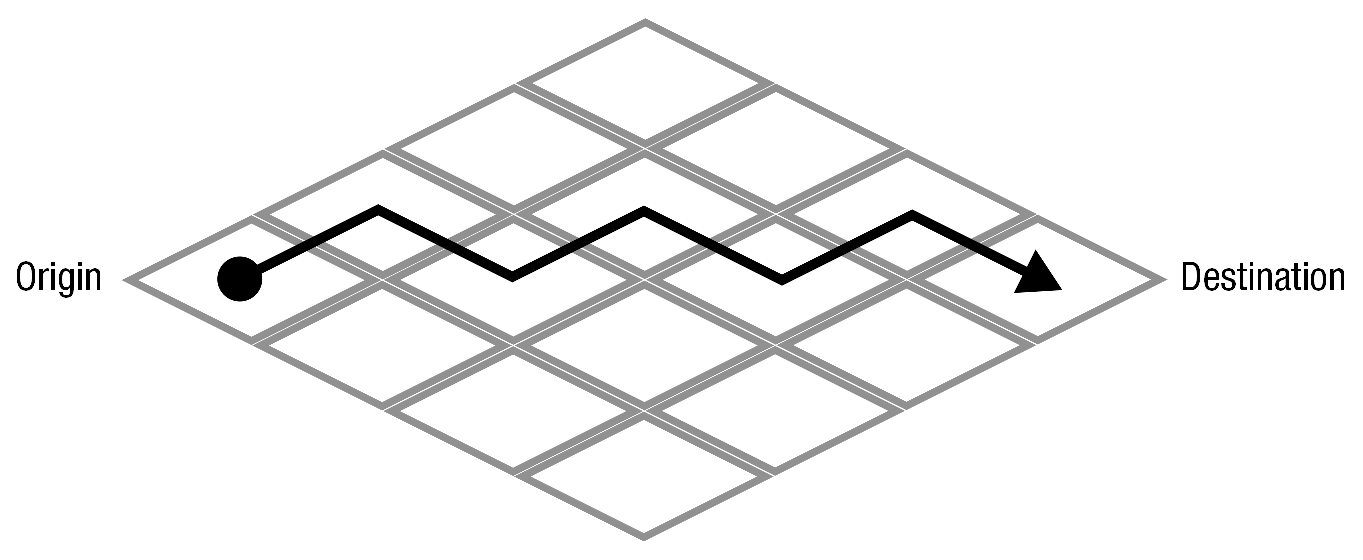
\includegraphics[width=8cm]{Images/manhattan_pathfind.eps}
    \caption{The Manhattan method in A* pathfinding.}
    \label{fig:manhattan_pathfind}
\end{figure}

The final reason was to do with collision detection and rendering. Because of the way collision detection works, entities crossing each other diagonally actually end up intersecting with each other, which is an ugly graphical artefact. As was discussed in section \ref{depth_limits} the work needed to make this a non-issue is considerable and there is little reason to allow for diagonal movement anyway.

While an entity handling direct input will find a path itself, those entities receiving input from the network instead get given a pre-determined path to follow. This is because it is possible for an entity to find a path on one client different from the path found on another. Although the game in its current form would not be overly affected by this, implementation of full interaction between entities could prove those differences disastrous. For example, a client may think it has the ability to interact with an entity, even though it actually does not.

If a frame was responsible for handling direct user input and generated a path and movement, an event is created to inform the server that the entity is going to move and to supply the path it is going to take to get to its destination.

% As an aside, currently, network input is simply taken from the client that created it and echoed by the server. Of course this is not ideal and in theory could produce terrible results due to malicious players. However, difficulties with the server implementation that are discussed in section \ref{server_implementation} will explain why it was done this way. That said, despite the less than ideal situation this represents, the client would still create paths for itself even if the server were to ultimately override them. This is because waiting for the server to respond with a valid path would be far too slow. Responsiveness of the game is very important, and a user having to wait several hundred milliseconds for their action to be translated to movement on the screen is completely unacceptable. The client therefore needs to be able to simulate the movement itself, with the server responding with a canonical path that the client can swap to using when it gets it.

\subsubsection{Following The Path}
The path returned from the A* algorithm is a series of tiles. To follow this path an entity first takes the next tile in the list and sets that as its destination. Whenever it reaches a destination, the path is checked again and a new destination selected. Once the path is completed there are no more destinations to get and the function does nothing. This following of the path is done every frame, regardless of whether there is input or not, and the path does not have to be generated anew every time a destination is reached.

To actually move towards a destination, the entity uses the \texttt{updatePosition()} function---the code for which can be found in Appendix B \ref{update_position}---which performs a series of checks to determine the entity's current location compared to its destination. When the direction of movement is established the entity's speed value is added to its position. This speed value is low, being just 0.125, taking eight frames to move an entire tile---though adjusting the speed value would allow an entity to move faster or slower.

\subsection{Game Master}
The Game Master has the special ability to select which character they want to control, though only characters which are not already controlled by another player. The introduction of this ability caused a lot of changes in the way entities are put together and handled and is the reason the \texttt{Player} class was merged back into the \texttt{Character} class, as discussed in Section \ref{entities_design}.

\subsubsection{Swapping Characters}
As mentioned at the end of Section \ref{input_implementation}, the Game Master can swap between characters by holding the shift key and clicking on an uncontrolled character entity. To handle this feature the \texttt{Character} class has two important methods---\texttt{processInput} and \texttt{updatePathing}---that can be swapped out depending on whether the entity is under player control or not.

The functionality to swap the methods out is implemented by making use of the fact that JavaScript functions can be stored in variables. Global variables are set containing the functions used. Swapping between them is handled using the input components that are assigned to \texttt{processInput}. For example, the \texttt{CharacterInputComponent}, shown in Listing \ref{characterinputcomponent}, handles the Game Master taking control of the entity.

\noindent
\begin{minipage}{\linewidth}
\begin{lstlisting}[style=js, caption={Input component for handling server input applied to non-player-controlled characters.}, label=characterinputcomponent]
var CharacterInputComponent = function(entity) {
    while (entity.eventQueue.length != 0) {
        var input = entity.eventQueue.pop();

        if (input.type === "server_move" && input.data.entity_id === entity.id) {
            return {"input": input.data.path};
        } else if ((input.type === 'change_entity' || input.type === 'server_change_entity') && input.data.x === entity.x && input.data.y === entity.y && !entity.user) {
            // GM changing to this entity
            entity.user = USER.id;
            entity.updatePathing = PlayerPathingComponent;
            entity.processInput  = PlayerInputComponent;
        }
        return false;
    }
};
\end{lstlisting}
\end{minipage}

As can be seen, this function handles the case where a non-player-controlled entity is given a movement command, but it will also handle the case where the Game Master is taking control of it. It does this by assigning the user attribute on the entity to the user ID of the Game Master, and then changing the \texttt{updatePathing} and \texttt{processInput} methods to use components designed to handle the direct input from a player. \texttt{PlayerInputComponent} handles the case where a Game Master is swapping to another entity instead by unsetting the user ID and changing the methods back to the character components.

\subsection{Issues With Input and Movement}
Input and movement as features were actually relatively smooth to implement, in comparison to the graphics and server code. However, they were not without their share of problems.

Input handling mostly caused problems due to taking a few iterations to work out the correct calculations to convert between the various different coordinate spaces. However, this is was mostly an issue of delaying further implementation, rather than a serious problem. The only noticeable bug to come from input handling itself was a subtle one, where click coordinates were shifted on the x axis by half a tile. This was solved by subtracting a half tile width from the click coordinate, as seen in previous Listing \ref{canvas_click_coordinates}.

Movement posed a bigger challenge. The first problem was with the A* pathfinding library. Or rather, the problem was with a mismatch between the meaning of x and y in the game engine, and x and y in the library. In the game engine, y represents a column of tiles, with x representing the rows. However, in the A* library, this was the other way around.

Initially the problem was not noticed, as clicking a tile would still have the player entity move to it. However, subtle problems existed that became more obvious as further testing was done. The most obvious problem was that the pathfinder seemed to think entities were in places they were not. This meant that the player entity was finding paths that had it moving through other entities on the map, and avoiding empty spaces. The other problem was that, on the rectangular test map, the bottom part was unusable. Both of these problems were caused by the pathfinder's representation of the game world being rotated 90° compared to the game engine's representation.

The initial attempt to solve this problem was to change the game engine, rather than the library. This worked in some ways, with the terrain rendering correctly, at least. However, the rest of the game world became even more broken, with input failing to work at all. Ultimately, the solution was to go into the library and flip references to x and y. This didn't take very long, but it did fix all problems that the mismatch had caused.

The second problem movement had was with the code used to actually move an entity, seen in Appendix B \ref{update_position}. Initially this code produced very odd results, with entities moving in multiple directions at once directly towards its end goal and occasionally getting stuck in a jittery state just before stopping in a tile.

The first problem was actually caused by a misunderstanding of the JavaScript array API. For some reason it was assumed the \texttt{pop()} function got the first result in the list, rather than the last. This was solved by changing the call to \texttt{pop()} with a call to \texttt{shift()} instead. The second issue was caused by a case where the addition of the speed value was causing the entity to slightly overshoot its target. On the next frame, the entity would then move backwards by the same amount, then move forwards again on the frame after that. This would repeat endlessly, leaving the entity stuck jittering in place. That was solved by checking to see whether the addition of the speed value to an entity's position would cause it to overshoot its target. If that happened, the entity instead sets its position to its destination, making sure it cannot get stuck.

\section{The Server}\label{server_implementation}
The server was, in theory, to be no more difficult to implement than the client. Indeed, some of the server-side code was going to just be a Python version of code already written for the client. After that, features like combat would have their logic implemented entirely server-side so there was no more duplication of functionality across them both, with the client being something more like a dumb view into the server.

Unfortunately, reality proved this theory to be badly false. The server took up an enormous amount of time, implementing things that had nothing to do with the game logic. Instead, handling the networking aspect as well as the management of the games themselves proved to be an incredible amount harder than expected. This was combined with the realisation that Python and JavaScript are very different languages, and even the code that was supposed to be replicated across the two proved more difficult to implement than anticipated.

This section will detail how the server works, handling connections with the client, the management of the multiple games that need to run at once and how the game logic is implemented server-side. The difficulties faced in doing these things will also be covered in detail.

\subsection{Connecting Clients}
The primary purpose of the server in the game is to provide a way of connecting clients together and thus allow people to play the game with each other. To achieve this there needs to be a way of managing those connections and passing messages between the clients.

Being a web-based game, the server is responsible for other things too. In particular it needs to be able to get players to the game in the first place, and to that extent is responsible for handling a lot of the UI and infrastructure that lets players log into the game, find games to join, and run games they have already joined.

To handle these aspects a framework was used, called Flask. Flask is ``microframework'', which provides built-in functionality to handle the routing of HTTP connections and the rendering of HTML templates. Further functionality is provided through extensions to the framework, which in this project provide database access and websockets, as well as a way of handling forms containing user input.

\subsubsection{HTTP Routing}
The majority of the routing work on the server-side is the handling of HTTP connections. This includes logging in and out, and finding and joining games. These routes also contain a lot of logic for managing games, with more detail on that in section \ref{managing_games}.

The first responsibility HTTP routing has is logging players in and out. This is handled in a standard way for web applications, having a database table containing usernames and hashed passwords. When a user logs in they provide an email address and password combination in a form, which is POSTed to the server for validation. An extension to the Flask framework is used to manage the hashing of passwords and the validation of user accounts. If the validation passes, a session cookie is set that keeps the user logged in.

The route for a login can be seen in Listing \ref{login_route}.

\noindent
\begin{minipage}{\linewidth}
\begin{lstlisting}[style=py, caption={Route for handling logins on the server-side.}, label=login_route]
@app.route('/login', methods=['GET', 'POST'])
def login():
    from forms import LoginForm
    form = LoginForm()

    if request.method == 'GET':
        return render_template('login.html', form=form)

    elif request.method == 'POST':
        if form.validate() == False:
            return render_template('login.html', form=form)
        else:
            session['email']    = form.email.data
            session['username'] = User.query.filter_by(email = session['email']).first().username
            session['user_id']  = User.query.filter_by(email = session['email']).first().id
            session['active_games'] = {}

            return redirect(url_for('gamelist'))
\end{lstlisting}
\end{minipage}

Routing in Flask works by having a decorator, seen on line 1, that defines the URL that applies to the function that follows it. The decorator defines the URL relative to the root, so in this case the full route for \texttt{/login} would be \texttt{example.com/login}. The route can also define which HTTP `verbs' it wants to handle. By default it handles only GET requests, but further ones can be defined as seen here.

The function itself can do anything. In this case, the function first imports a form class, which is used to define the data the incoming request will have, like an email and a password. Next, the route checks to see whether it is being called from a GET or a POST request. If GET, it just returns the form for the user to fill out; if POST, it validates a form coming in and does something based on the result of that validation. A failed validation will display the login form again and a successful validation will create a new user session and redirect the user to their list of games.

All routes to some extent follow this pattern, depending on their purpose, with some having the very important responsibilities of creating games or letting a user join an already existing game.

\subsubsection{Socket Routing}
The other type of routing the server does is that of websockets. To achieve this an extension for Flask is used, which implements the SocketIO library. Currently there are three types of event handled by sockets: movement, connection and disconnection.

\noindent
\begin{minipage}{\linewidth}
\begin{lstlisting}[style=py, caption={Socket for passing movement events between clients and server.}, label=movement_socket]
@socketio.on('player_move', namespace = '/game')
def player_move(data):
    if data['game_id']:
        running_games[data['game_id']]['input_queue'].put({'type': 'player_move', 'input': data})

    emit('server_move', data, room = data['game_id'])
\end{lstlisting}
\end{minipage}

Listing \ref{movement_socket} shows the socket responsible for passing movement around between clients and informing the server. As can be seen, there is a decorator responsible for defining what the route is, followed by a function to handle the route---the same as the HTTP routing. The difference is that this handles websockets using SocketIO, rather than handling HTTP connections.

The route is defined as being a socket name---in this case \texttt{player\_move}---and a namespace. The namespace means that there can be multiple sockets of the same name being passed around that do different things. As an example, if there were a socket called \texttt{message} that existed in two namespaces, \texttt{/game} and \texttt{/chat}, they would not interfere with each other.

This route's function has two purposes. The first is that it informs the server about the movement so that it can simulate it. How that is achieved is detailed in Section \ref{server_movement}. The other purpose is to then inform the clients connected that a movement has occurred, using the \texttt{emit} function. This emits a socket message that contains the data about the movement, in this case which entity moved and the path it is taking to do so.

To make sure that clients don't receive messages that are from different games, the concept of a room is used. These rooms are provided by the SocketIO library and contain a list of socket connections with the key being the game ID it relates to. Because the game ID is always sent with a socket message, the rooms can be used to make sure that only clients connected to that particular game will receive messages from it.

Connection and disconnection don't emit anything back to clients. Instead they simply inform the server-side game simulation that a user has connected or disconnected and leave it up to the game to decide what to do with that information. Section \ref{managing_games} details how this works.

\subsection{Managing Games}\label{managing_games}
As important as routing is to the functioning of the game, a huge amount of logic server-side has the responsibility of managing the games themselves. Managing the games refers to creating entirely new games, starting the game loop on the server and making sure players are placed into the right ones. This section will also deal with how games are shut down, which the game process itself is responsible for handling.

\subsubsection{Multiple Games And Threads}
One of the major reasons that the server-side proved more difficult to implement than expected was the necessity of running the game loop in a separate thread. The reason for this is that the game loop is blocking, which means that once it starts nothing else can run outside of it. If it were not run in a separate thread the server simply wouldn't function.

To handle the threading functionality the game loop is contained within a class called \texttt{GameLoop}, which inherits from the class \texttt{threading.Thread}. The constructor for \texttt{GameLoop} first calls the superclass' constructor to activate the threading capabilities, and then continues with its own constructor.

The constructor in \texttt{GameLoop} does a few things. Firstly it creates instance variables linking it to the queues used to communicate with the router and then goes on to create the entities in the game that it needs to keep track of. For threading the entities don't matter very much as they are kept in an \texttt{entities} variable in the class itself. However, the queues are important; without the queues the game loop would be isolated and never do anything because it couldn't receive any input.

The queues are instances of the Python \texttt{Queue} class and are created by the router when it first starts up a new game loop process. They are then passed into the \texttt{GameLoop} constructor and also kept around in the router so it can use them too. There are two queues, one for input from the router and one for sending information back out, known as \texttt{input\_queue} and \texttt{reply\_queue}. The input queue is read by the game loop every frame to check for messages it needs to handle. The reply queue is only used in specific circumstances when the router expects to get a response. Because the router cannot have its own loop and still function correctly there is no reasonable way to regularly check for replies from a game. This means that the game loop can only respond to input and cannot generate events by itself because those events would never get seen. Luckily, this isn't such a big issue for the game as there is no AI aspect to generate events without player input.

Finally, the game loop sets a variable called \texttt{alive}, used by the game loop itself to keep running. When the variable is unset the loop will stop running and the thread will end. Starting the thread, however, is done by the router calling a method called \texttt{start()}, inherited from the \texttt{Thread} superclass, which calls the \texttt{run()} method defined in \texttt{GameLoop}.  If \texttt{run()} is called directly a new thread won't be started, which will cause the game loop to block the server.

Because there are multiple games running at once in separate threads it is necessary to have a a system in place that can manage those threads, starting them up and directing connecting players to the correct one. This functionality is given to the router, as all of these functions are responses to connections and requests made by users.

\subsubsection{Creating Games}
Before games can be started and joined, they first have to exist. From a game design point of view this is the starting point of the Game Master, but from a technical point of view it is the creation of a basic terrain and the addition of some entities to the world.

Game creation is started from the route \texttt{/game/create}. A user would get here by clicking a link on their game list page. They then proceed to enter a name for the new game they are creating and hit submit. Once the form is submitted with the new name the route proceeds to create a pre-defined, default world with a small map and three entities---two walls and a userless character that the Game Master can take control of. The map and these entities are committed to the database and the user that created the game is set as the Game Master for it, gaining whatever privileges that entails.

\subsubsection{Starting And Joining Games}
Starting up and joining a game come from the same route, seen in Listing \ref{game_route}.

\noindent
\begin{minipage}{\linewidth}
\begin{lstlisting}[style=py, caption={The route responsible for starting a game thread.}, label=game_route]
@app.route('/game/<path:id>')
def game(id):
    if 'email' not in session:
        return redirect(url_for('login'))

    current_game = Game.query.filter_by(id = id).first()

    session['active_games'][id] = True

    import game, Queue
    if id not in running_games:
        scene = Game.query.filter_by(id = id).first().current_scene
        entities = Entity.query.filter_by(scene = scene).all()
        input_queue = Queue.Queue()
        reply_queue = Queue.Queue()

        running_games[id] = {'game': game.GameLoop(entities, scene, input_queue, reply_queue), 'input_queue': input_queue, 'reply_queue': reply_queue}
        running_games[id]['game'].start()

    return render_template('game.html', current_game = current_game)
\end{lstlisting}
\end{minipage}

When a player decides to join a game, they go to this route, the URL being in the form \texttt{/game/<id>}, with \texttt{id} representing the game ID they wish to join. The route first checks to see if the user is logged in and, if so, it goes to the database to get the game from that ID. The final step before actually handling the game starting itself is to add the game to the user's session. This is necessary to handle disconnect events as will be seen in Section \ref{disconnecting}.

The next part deals with starting a game. First, the \texttt{running\_games} variable is checked to see if the game is already active. This is a global variable held by the router and is different from the session variable linked to each individual user.

If the game already exists the route just returns the page that runs the game in the client. If a user is the first to try and join the game, however, then the game needs to be started up. To do this the router first gets the current scene and then the list of entities linked to that game from the database, followed by the two queues it needs to communicate with the game loop once it's running. It then creates a new entry in the \texttt{running\_games} list, and in doing so creates a new instance of the \texttt{GameLoop} class, passing in the scene, entities and queues. It also attaches the queues to the \texttt{running\_games} list so that it can get them later. Finally, the game is started and it then renders the page containing the game for the user.

To actually get game information to the client another route is needed. This route gets what is known as the scene, which contains the map and the entities that are in the game. The full code for this route can be found in Appendix B \ref{scene_route}.

The route first checks to see if the game is running. If so, it asks the game to return its current state. Doing this means that clients that are connecting after the game has started are getting the state of the game as it currently is, rather than what was previously persisted to the database. However, it still needs to grab information from the database about entities because not everything is kept in the server-side state, such as an entity's sprite. It then goes through every entity and makes sure it has the current information instead of the old persisted information and then packages it all up as JSON to send back to the client.

The final step of joining a game is the client sending a socket message called \texttt{game\_loaded}. Upon receiving this event the server-side game is informed that a new user has connected and the user is added to the socket room for that game.

\subsubsection{Disconnecting}\label{disconnecting}
In theory disconnecting is a simple part of the implementation, especially as SocketIO provides disconnect events itself. However, in reality the disconnection of users proved to be one of the most challenging parts of the server implementation, primarily because of the game being hosted in a browser and the need for empty games to be shut down automatically so as not to leave unused threads lying around.

Individually neither problem is particularly hard to solve. Together, though, they are a serious issue, and one that was not at all foreseen. The issue stems from the fact that when running a game from a browser users can refresh the page. This causes a disconnect event but in reality the user only replaced their old connection with a new one. Worse, the disconnect event is delayed, sometimes for up to 15 seconds, due to SocketIO only noticing a disconnect has occurred when a client fails to reply to a heartbeat check. When keeping track of how many users are connected to a game to know if it is necessary to shut it down, this fact can cause a player to end up in a situation where the game server isn't actually running even though they are supposedly playing the game.

The first step to solving these issues is to get the disconnect event itself. This is handled through a built-in socket message called \texttt{disconnect}, provided by SocketIO. It is at this point that the storing of the active game in the user's session becomes necessary, as the disconnect event cannot carry extra information, such as what game the disconnect is relevant to. When this event is received, the router passes it along to the game, which is keeping track of all the users currently connected to it.

Because users can refresh the page and thus create false disconnects, when adding a player to a game the game keeps a count, which is incremented whenever a player add event occurs. When a user disconnects, their count is decremented instead. This has the effect of keeping track of the difference in connection events and disconnect events, so that when the disconnect events come through they are not taken to mean the user has actually disconnected.

If the user connection count does happen to reach 0 and the user in question is the only one connected then the server will proceed to shut itself down. This is done by unsetting the \texttt{alive} flag, which will stop the game loop from running the next frame. Once this is done the game proceeds to ask every entity in it to perform its own shutdown function, which has the entities make sure they are on a whole tile rather than transitioning between tiles. Afterwards the entity is persisted to the database so that its state can be saved for the next time the game is loaded.

When all this is done the thread has nothing left to do and so it stops itself. The next time a user attempts to connect to the game it will go through the process of starting up again.

\subsection{The Server-side Game}\label{server_movement}
Although figuring out the management of the games took up most of the time dedicated to the server-side---and ultimately the project in general---the game still runs and there is logic dedicated to actually getting the game to function properly.

Mention has already been made of the \texttt{GameLoop} class and its role in handling the management of the games, both directly and in terms of forcing certain decisions to be made. However, no mention has been made of exactly how it works, particularly with respect to its differences with the client-side loop.

As mentioned in Section \ref{game_loop_implementation}, the client-side game loop is implemented in a non-blocking way. The server-side doesn't operate in the same way as Python does not, by default, run inside an event loop like JavaScript does. There are ways to implement one using libraries such as Twisted \cite{citeulike:13161624}, but it is not easy. Instead, the server-side uses a traditional \texttt{while} loop and thus takes complete control of the thread. This primary loop operates as long as the \texttt{alive} variable---described in the previous section---is set.

Like the client the server game loop keeps track of lag time between frames to make sure that the game simulation doesn't fall behind. However, the server also relies on this timing information to make sure frames are updated at the correct interval so that they don't run too fast either.

During a frame the server checks the input queue, filled by events from the router. The events that it can handle directly are for adding or disconnecting players, returning the entities it has running for the sake of a newly connected user, as well as an event to manually stop the thread. The functioning of these is discussed in the previous section. If none of these events is relevant the loop passes the input onto the entities in the game, calling each entity's own update function. This is the same concept as used in the client-side to handle frame updates.

The entities on the server-side function in a similar way to the client-side, though unfortunately their functionality is slightly reduced as they cannot find paths for themselves, which means that they cannot act as the canonical version of the game state they are supposed to be. Although adding a pathfinder to the server-side would not be too difficult a problem---simply being a case of adding a library similar to the client-side---it is not quite as simple to make sure the client receives these new paths and handles them smoothly, and time ran out dealing with the rest of the server. Despite the lack of ability to create their own paths, however, entities on the server are able to follow paths given to them from clients and handle their movement between tiles in exactly the same manner as the client. This allows the server to at least offer up the game state to newly connecting or refreshing clients, even in the case of entities being in the middle of moving.

\section{Planned \& Implemented Features}
As can likely be gathered from this chapter, many of the features planned in the minimal system were not implemented by the end of the project. In particular, combat and chat are not present, with combat being the more egregious omission. The biggest reason for the lack of minimal system completion is the server taking up a lot more time than expected due to all the problems related to multiple games and threading.

However, despite these problems a good number of the features are in place, and much of what isn't done can be added onto the groundwork already laid with little issue.

% The implementation should look at any issues you encountered as you tried to implement your design. During the work, you might have found that elements of your design were unnecessary or overly complex; perhaps third party libraries were available that simplified some of the functions that you intended to implement. If things were easier in some areas, then how did you adapt your project to take account of your findings?

% It is more likely that things were more complex than you first thought. In particular, were there any problems or difficulties that you found during implementation that you had to address? Did such problems simply delay you or were they more significant?

% You can conclude this section by reviewing the end of the implementation stage against the planned requirements.
